%\subsubsection{Simulation:Experiment Resolution Matching}

The detector responses in the GEMC system were modeled to perform slightly better than their real-world counterparts. This means the signal data from the simulations are cleaner than the real experiment, and so smearing factors must be added to provide a better match. This convention was chosen because the alternative (with simulations performing worse than real-world detectors) would yield data that is difficult to deconvolve. \figref{fig:bad} shows the discrepancy between the experimental and simulated data sets, for various variable combinations. 

\begin{figure}[hbt]
	\centering
	\includegraphics[page=125,width=0.3\linewidth]{Chapters/Ch4-BaseAnalysis/0_preprocessing/0_B_simulation_data_preprocessing/pics/nosmear/outbending_rad_All_All_All_no_smearingME_epgg_exp_vs_sim.png}
	\includegraphics[page=123,width=0.3\linewidth]{Chapters/Ch4-BaseAnalysis/0_preprocessing/0_B_simulation_data_preprocessing/pics/nosmear/outbending_rad_All_All_All_no_smearingMM2_egg_exp_vs_sim.png}
	\includegraphics[page=128,width=0.3\linewidth]{Chapters/Ch4-BaseAnalysis/0_preprocessing/0_B_simulation_data_preprocessing/pics/nosmear/outbending_rad_All_All_All_no_smearingMM2_epgg_exp_vs_sim.png}
	\includegraphics[page=130,width=0.3\linewidth]{Chapters/Ch4-BaseAnalysis/0_preprocessing/0_B_simulation_data_preprocessing/pics/nosmear/outbending_rad_All_All_All_no_smearingMM2_ep_exp_vs_sim.png}
	\includegraphics[page=133,width=0.3\linewidth]{Chapters/Ch4-BaseAnalysis/0_preprocessing/0_B_simulation_data_preprocessing/pics/nosmear/outbending_rad_All_All_All_no_smearingMpi0_exp_vs_sim.png}
	\includegraphics[page=135,width=0.3\linewidth]{Chapters/Ch4-BaseAnalysis/0_preprocessing/0_B_simulation_data_preprocessing/pics/nosmear/outbending_rad_All_All_All_no_smearingMPt_exp_vs_sim.png}
	
	\caption[Simulation and Experiment Matching before Smearing]{Comparison of experiment (blue) and simulation (red) missing mass, energy, momentum, and invariant gamma-gamma mass distributions, before any smearing factors were added to the simulation data.}
	\label{fig:bad}
\end{figure}


To improve the matching between simulation and experiment, Gaussian smearing factors were added after reconstruction to the simulated dataset. These factors were tuned by S. Lee \parencite{Lee2022MeasurementDetector} to have optimal matching across all missing mass spectra combinations as shown in \figref{fig:good}. In particular, the outgoing proton and photon momenta were smeared with Gaussian kernels with standard deviations $\sigma$ determined as function of momenta and dependent on particle location (CD, FD, or FT).

\begin{figure}[hbt]
	\centering
	\includegraphics[page=125,width=0.3\linewidth]{Chapters/Ch4-BaseAnalysis/0_preprocessing/0_B_simulation_data_preprocessing/pics/yessmear/outbending_rad_All_All_All_for_aps_2022_plots_sangcutsME_epgg_exp_vs_sim.png}
	\includegraphics[page=123,width=0.3\linewidth]{Chapters/Ch4-BaseAnalysis/0_preprocessing/0_B_simulation_data_preprocessing/pics/yessmear/outbending_rad_All_All_All_for_aps_2022_plots_sangcutsMM2_egg_exp_vs_sim.png}
	\includegraphics[page=128,width=0.3\linewidth]{Chapters/Ch4-BaseAnalysis/0_preprocessing/0_B_simulation_data_preprocessing/pics/yessmear/outbending_rad_All_All_All_for_aps_2022_plots_sangcutsMM2_epgg_exp_vs_sim.png}
	\includegraphics[page=130,width=0.3\linewidth]{Chapters/Ch4-BaseAnalysis/0_preprocessing/0_B_simulation_data_preprocessing/pics/yessmear/outbending_rad_All_All_All_for_aps_2022_plots_sangcutsMM2_ep_exp_vs_sim.png}
	\includegraphics[page=133,width=0.3\linewidth]{Chapters/Ch4-BaseAnalysis/0_preprocessing/0_B_simulation_data_preprocessing/pics/yessmear/outbending_rad_All_All_All_for_aps_2022_plots_sangcutsMpi0_exp_vs_sim.png}
	\includegraphics[page=135,width=0.3\linewidth]{Chapters/Ch4-BaseAnalysis/0_preprocessing/0_B_simulation_data_preprocessing/pics/yessmear/outbending_rad_All_All_All_for_aps_2022_plots_sangcutsMPt_exp_vs_sim.png}
	
	\caption[Simulation and Experiment Matching after Smearing]{Comparison of experiment (blue) and simulation (red) missing mass, energy, momentum, and invariant gamma-gamma mass distributions, with smearing factors added to the simulation data proton and photon momenta.}
	\label{fig:good}
\end{figure}